% !TEX root = ../main.tex
% SECTION 4: TOLERANZEN
% Inhalt: Liv Erne, Silvio Seiz — Form: ZSF-Template-Rework
% ============================================================

\StartChapterOnNewColumn[ch:toleranzen]{Toleranzen}
\ZSFindex{Toleranz}

\begin{runintext}
\ZSFmuted{Bei $\ZSFtolD = 80$ wird der Tabellenabschnitt $50 - 80$ gewählt, da bis und mit gilt.}
\end{runintext}

\SubsectionBar[sec:toleranzfeldbilder]{Toleranzfeldbilder}
\ZSFindex{Toleranzfeldbild}
\ZSFindex{Passung}

\begin{runintext}
Kombinationen der Toleranzfelder von Welle und Bohrung können \ZSFkeyword[Spielpassung]{Spiel-}, \ZSFkeyword[U@Übergangspassung]{Übergangs-} und \ZSFkeyword[U@Übermasspassung]{Übermasspassungen} erzeugen:
\end{runintext}

\begin{figbox}[Spiel- / Übergangs- / Übermasspassung]
\centering
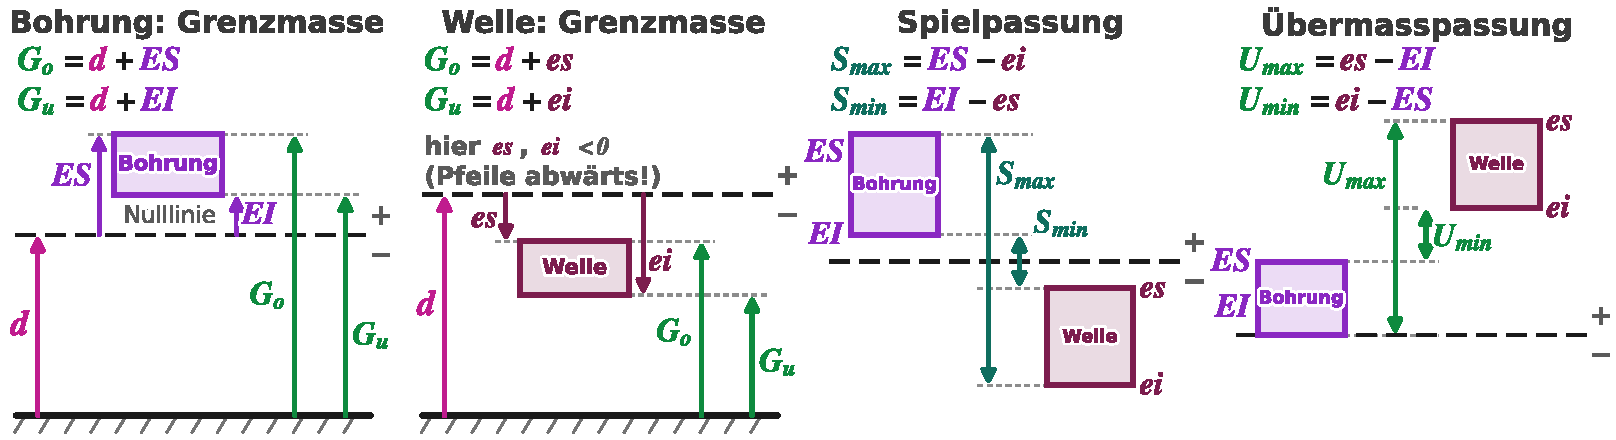
\includegraphics[width=0.88\linewidth,keepaspectratio]{graphics/toleranzfelder.pdf}
\end{figbox}

\begin{factlist}
\ZSFFact{Spielpassung}{$\ZSFtolSmin > 0 \ (\ZSFtolSmin = \ZSFtolEI - \ZSFtoles)$}
\ZSFFact{Übermasspassung}{$\ZSFtolSmax < 0 \ (\ZSFtolSmax = \ZSFtolES - \ZSFtolei)$}
\ZSFFact{Übergangspassung}{$\ZSFtolSmin < 0 < \ZSFtolSmax \ (\ZSFtolSmin = \ZSFtolEI - \ZSFtoles, \ZSFtolSmax = \ZSFtolES - \ZSFtolei)$}
\end{factlist}

%Beispiel Toleranzfeldbild:
%\ZSFfig{graphics/v6_toleranzzeichnung_welle.png}{Toleranzzeichnung Welle}{}

\begin{factlist}
\ZSFFact{Welle}{Oberes Abmass $\ZSFtoles$, unteres Abmass $\ZSFtolei$ ($\ZSFtoles > \ZSFtolei$)}
\ZSFFact{Bohrung}{Oberes Abmass $\ZSFtolES$, unteres Abmass $\ZSFtolEI$ ($\ZSFtolES > \ZSFtolEI$)}
\end{factlist}
\ZSFindex{Abmass}

\begin{formulabox}[Übermass $\ZSFtolU$ und Spiel $\ZSFtolS$]
\formulasources{$\ZSFtolUwMinMax$:~\ZSFsource{aus}{formula:tol-uw} \ $\cdot$ \ $\ZSFtolG$:~\ZSFsource{aus}{sec:rautiefe}}
\[ \ZSFtolUmin = \ZSFtolUwMin + \ZSFtolG = \ZSFtolei - \ZSFtolES = \ZSFtolei - (\ZSFtolEI + \ZSFtolIT) \]
\[ \ZSFtolUmax = \ZSFtolUwMax + \ZSFtolG = \ZSFtoles - \ZSFtolEI = (\ZSFtolei + \ZSFtolIT) - \ZSFtolEI \]
\[ \ZSFtolSmin = \ZSFtolEI - \ZSFtoles \qquad \ZSFtolSmax = \ZSFtolES - \ZSFtolei \]
\formulasep
\[ \ZSFtolEI = \ZSFtolES - \ZSFtolIT \qquad \ZSFtolei = \ZSFtoles - \ZSFtolIT \]
\formulanote{$\ZSFtolUwMinMax$:~wirksames Übermass \ $\cdot$ \ $\ZSFtolG$:~Glättung}
\end{formulabox}

\begin{figbox}[Toleranzen]
\centering
$\vcenter{\hbox{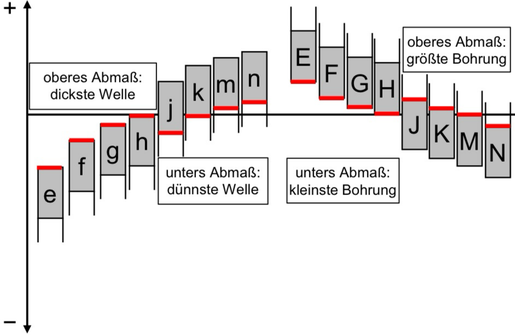
\includegraphics[width=0.62\linewidth,keepaspectratio]{graphics/toleranzfeld_lage_abmasse.png}}}%
\vcenter{\hbox{\begin{minipage}[c]{0.34\linewidth}
\centering
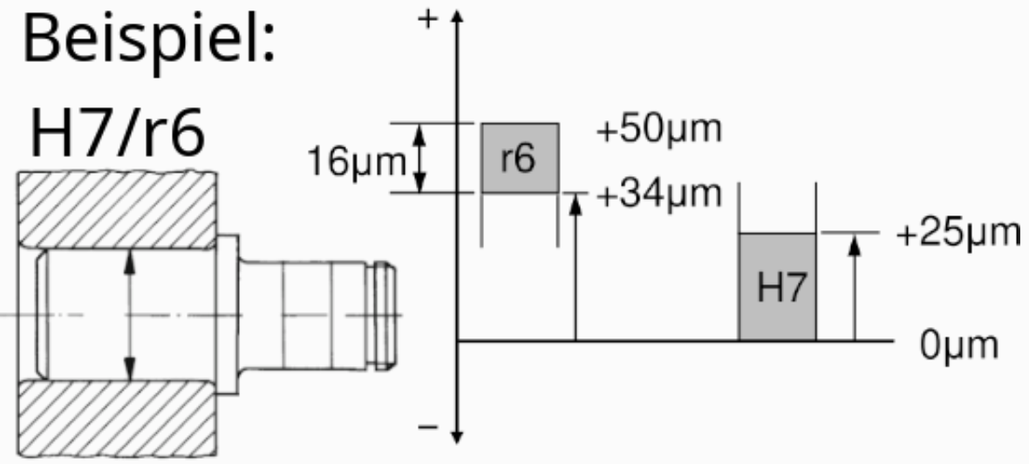
\includegraphics[width=\linewidth,keepaspectratio]{graphics/toleranzen_beispiel_h7r6.png}

\ZSFgapS
{\ZSFReadableOn Grundtoleranzgrade $\ZSFtolIT$ (Nummer nach Buchstabe) bestimmt wie gross das \textcolor{HighlightRed}{Feld} ist.\par}
\end{minipage}}}$
\end{figbox}

\phantomsection\label{formula:tol-uw}
\begin{formulabox}[Wirksames Übermass]
\formulasources{$p_{\min}$:~\ZSFsource{aus}{sec:zpv} oder \ZSFsource{aus}{sec:kpv}}
\formulanoteabove{%
$p_{\max}$:~Grenze aus zulässiger Bauteilspannung.}
\[ \ZSFtolUwMinMax = \dfrac{\ZSFtolPMinMax \cdot \ZSFtolDF}{\ZSFtolEA} \cdot \ZSFtolK \]
\formulanote{$\ZSFtolPMinMax$:~min./max. Fugenpressung \ $\cdot$ \ $\ZSFtolK$:~Hilfsgrösse \ $\cdot$ \ $\ZSFtolDF$:~Fugendurchmesser \ $\cdot$ \ $\ZSFtolEA$:~E-Modul des Aussenteils (Nabe)}
\end{formulabox}
\ZSFindex[ubermass, wirksames]{Übermass, wirksames}

\begin{warnbox}[Übermass vs. Spiel]
\ZSFconclusion{Zerbrechen bei zu grossem Übermass (Spannungen)}

\ZSFconclusion{Durchrutschen bei zu viel Spiel (keine Drehmomentübertragung)}
\end{warnbox}

\SubsectionBar[sec:hooke]{Hooke'sches Gesetz}
\ZSFindex{Hooke'sches Gesetz}

\begin{formulabox}
\formulasources{$\ZSFtolE$:~\ZSFsource{aus}{sec:werkstoffkennwerte}}
\[ \ZSFtolSigma = \ZSFtolE \cdot \ZSFtolEps = \ZSFtolE \cdot \dfrac{\ZSFtolDeltaL}{\ZSFtolL} \qquad \ZSFtolDeltaL = \dfrac{\ZSFtolSigma \ZSFtolL}{\ZSFtolE} \qquad \ZSFtolDeltaD = \dfrac{\ZSFtolP \cdot \ZSFtolDF}{\ZSFtolEA} \cdot \ZSFtolK \]
\formulasep
\formulanoteabove{Unter Temperatureinfluss:}
\[ \ZSFtolDeltaL = \ZSFtolAlpha \cdot \ZSFtolL \cdot \ZSFtolDeltaT \]
\formulanote{mit Wärmeausdehnungskoeffizient $\ZSFtolAlpha$ in $\dfrac{1}{10^{-6}K}$.}
\end{formulabox}
\ZSFindex[warmeausdehnung]{Wärmeausdehnung}

\begin{runintext}
Andernfalls kann eine Kerbe mit Gummiring eingefügt werden, um das zusätzliche Spiel durch den Temperatureinfluss zu dämpfen.
\end{runintext}

\SubsectionBar[sec:rautiefe]{Gemittelte Rautiefe $\ZSFtolRz$ und Glättung $\ZSFtolG$}
\ZSFindex{Rautiefe}
\ZSFindex[glattung]{Glättung}

\begin{runintext}
Gestaltabweichungen (Formabweichungen, Welligkeit, Riefen und Rillen) werden beim Fügevorgang geglättet.
\end{runintext}

\ZSFfigside[0.60]{graphics/v6_surface_roughness_smoothing.png}{Glättung}{%
  \ZSFReadableOn
  {\centering $\displaystyle \ZSFtolRz = \dfrac{\ZSFtolZone + \ZSFtolZtwo + \cdots + \ZSFtolZn}{\ZSFtolN}$ \par}
  \ZSFgapS
  {\centering $\displaystyle \ZSFtolG = 0.4\cdot(\ZSFtolRzA + \ZSFtolRzI)$ \par}
}

\SubsectionBarOnNewColumn[sec:genauigkeit]{Genauigkeit}
\ZSFindex{Genauigkeit}
\ZSFindex[prazision]{Präzision}
\ZSFindex{Richtigkeit}

\begin{propertylist}[Genauigkeit]
\ZSFFact{Richtigkeit}{Nähe vom Mittelwert ($\ZSFtolMu$) zum Sollwert (Zielwert) $\rightarrow$ Systematische Fehler (Im Graphen verschiebt sich die Glockenkurve nach links/ rechts)}
\ZSFFact{Präzision}{Streuung um den Mittelwert, beschrieben durch die Standardabweichung ($\ZSFtolSigma$) $\rightarrow$ Zufällige Fehler (Im Graphen flacht die Glockenkurve ab und sie wird breiter)}
\ZSFFact{Genauigkeit}{Richtigkeit und Präzision $\rightarrow$ $\ZSFtolMu =$ Sollwert, $\ZSFtolSigma$ gegen Null}
\end{propertylist}
